\documentclass{article}

%package setup
\usepackage{graphicx}
\graphicspath{ {./images/} }
\usepackage{amsmath}
\usepackage{fancyhdr}
\usepackage[margin=1in]{geometry}
\usepackage{subcaption}
\usepackage{comment}
\usepackage[hidelinks]{hyperref}
\usepackage{enumitem}
\usepackage{float}
\usepackage{textcomp, gensymb}
\usepackage{caption}
\setlength\parindent{0pt}


\pagestyle{fancy}
\fancyhf{} % Clear header/footer settings
\rhead{\thepage} % Page number on the right in the header
\lhead{ASE 375 Final Project Proposal} % Your lab report title on the left

\begin{document}

\begin{titlepage}
  \centering
  
\includegraphics[height=2.5cm]{ase-logo-formal.png}  % Adjust the height as needed
  \vspace{1cm}  % Add some vertical space
 
  \Large \textbf{ASE 375 Electromechanical Systems}\\
  \large \textbf{Section 14115}\\
  \vspace{0.5cm}
  \textbf{Monday: 3:00 - 6:00 pm}\\
 
  \vspace{1cm}
 
  \hrule
  \vspace{0.5cm}
 
  \Huge \textbf{Final Project Proposal: \\
                Propeller Twist Efficiency}\\
  \Huge \textbf{}\\
 
  \vspace{0.5cm}
  \hrule
 
  \vspace{1cm}
 
  \normalsize \textbf{Group 6: Andrew Doty, Andres Suniaga, Dennis Hom}\\
  \normalsize \textbf{Due Date: 04/01/2024}
 
\end{titlepage}
\newpage

\section{Introduction}
Question: Imagine we want to design an RC aircraft. What is the most efficient propeller for our motor? Moreover, How does propeller twist affect efficiency?
\\[2mm]
Propeller twist defines the angle of attack of the blade of the propeller. Twist varies from the hub to the tip of the propeller due to the different speeds along the blade, but this twist allows for uniform lift throughout the propeller's blade.

\section{List of Equipment}
\begin{enumerate}
    \item Tension Link Load Cell, along with required connections and components
    \item BLDC Motor with the proper rated Brushless Electronic Speed Controller 
    \begin{itemize}
        \item Stator diameter and height to be determined.
        \item $\text{K}_{\text{v}}\; [\frac{
        \text{RPM}}{\text{V}}]$ to be determined .
    \end{itemize}
    \item Power Supply or 3-6S Lithium-Ion/Polymer battery with Voltmeter, Ammeter, and Watt-meter
    \item PWM Wave Generator or PWM/Servo Tester
    \item Two-Blade Propellers of different pitch
    \begin{itemize}
        \item Propeller diameter to be determined, based upon motor specifications.
    \end{itemize}
    \item Thrust Stand with mounting for BLDC Motor and Placement of Load Cell
\end{enumerate}

\section{Experiment}
How will we determine the propeller's efficiency? Using a thrust stand designed to mount our BLDC Motor, we will measure the thrust force and the power used. The load cell shall be placed underneath the motor on the stand and will measure the force of thrust as shown in Figure \ref{fig:finalsetup}. We will keep track of the input voltage, current, and power from the power supply, which shall read out these electrical quantities.
\begin{figure}[H]
    \centering
    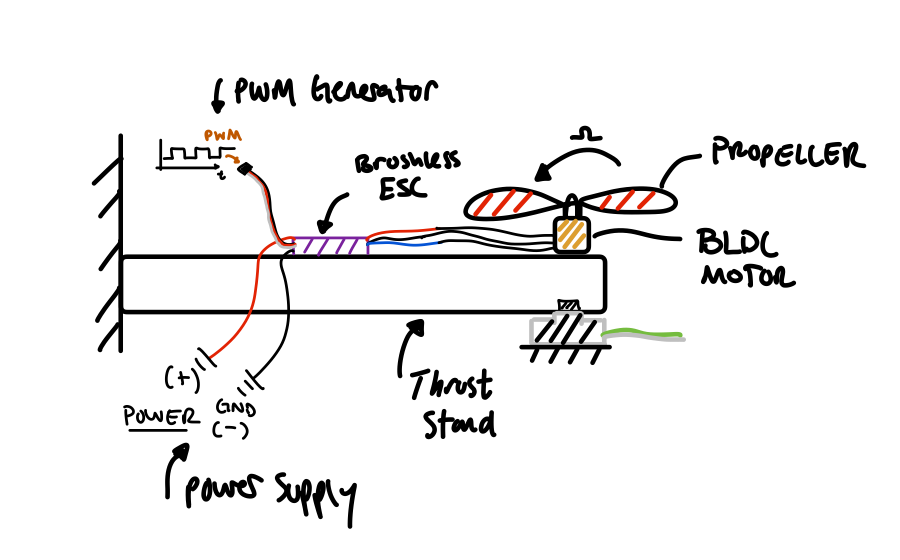
\includegraphics[width = 0.5\textwidth]{EMech_FinalExperiment_IdeaSetup.png}
    \caption{Hypothetical Experiment Setup}
    \label{fig:finalsetup}
\end{figure}
We will experiment with propellers of different twist but same diameter. With the data gathered from the load cell and power consumption, we shall determine the propeller efficiency by $\eta_{p} = \dfrac{F_{T}\, V}{P}$, where $F_{T} = \; \text{Thrust}$, $P = \; \text{Electrical Power}$, and $V = \; \text{Flight Velocity}$. We will normalize this efficiency parameter by $V$, assuming a constant theoretical flight velocity. The propeller with the highest $\eta_{p}$ will be the chosen propeller for our RC aircraft.
\newpage

\end{document}
